\documentclass[11pt]{article}

\usepackage{mathtools}
\usepackage{hyperref}
\usepackage{xepersian}
\settextfont{XB Zar}
\setlatintextfont{Linux Libertine}
\usepackage{graphicx}
\usepackage{csquotes}
\title{\textbf{نتایج تحلیل داده‌های مربوط به بلاگ}}
\author{محمدمهدی جهان‌آرا، عرفان لقمانی}
\date{\today}
\begin{document}

\maketitle

\section{داده‌ها}
مطالعه‌ای روی وبلاگ‌های دامنه‌ی blog.ir انجام دادیم. ابتدا شبکه‌ای که در آن هر راس یک وبلاگ و یال‌ها لینک‌‌های یک وبلاگ به وبلاگ دیگر است ساختیم به این روش که از تعدادی راس شروع کرده و با BFS رئوس دیگر را اضافه کردیم تا مولفه‌ها تمام شود.
تا اینجا:
\begin{center}
\begin{tabular}{|c|c|}
\hline
راس & 18050 \\
یال & 42743 \\
\hline
\end{tabular}
\end{center}
به‌دست آمده است که در
\href{http://198.143.180.155/blog}{این آدرس}
قابل مشاهده است. وبلاگ‌ها با درجه‌ورودی، درجه خروجی، ضریب خوشه‌بندی و تعداد بلاگ‌هایی که از آنها می‌توان به این بلاگ رسید مرتب شده اند.
هم چنین برای هر بلاگ آخرین پست، گراف پیرامون آن بلاگ تا دو عمق و لیست بلاگ‌های ورودی و خروجی آن را نمایش می‌دهیم برای مثال:
\href{http://198.143.180.155/blog/blog/acm}{بلاگ acm}
\section{نتایج}
\lr{
\begin{center}
\begin{tabular}{|c|c|c|c|c|c|c|c|}
\hline
Network & N & L & <k> & $<k_{in}^2>$ & 
$<k_{out}^2>$ & $\gamma_{in}$ & $\gamma_{out} $\\
blogs & 18050 & 42743 & 2.368 & 205.846 & 54.100 & 2.32 & 3.49 \\
\hline
\end{tabular}
\end{center}
}
\begin{figure}[!h]
\caption{توزیع درجه خروجی}
\centering
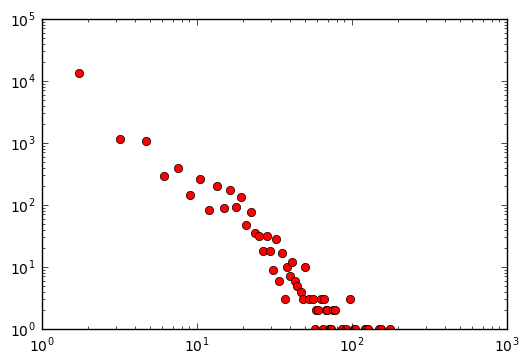
\includegraphics[height=0.4\textheight]{out-degree-distribution}
\end{figure}
\begin{figure}[!h]
\caption{توزیع تجمعی درجه خروجی}
\centering
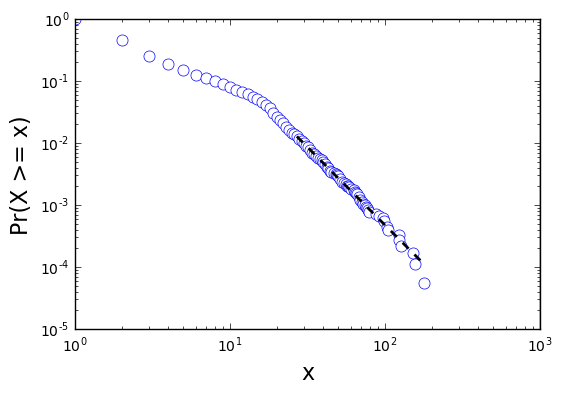
\includegraphics[height=0.4\textheight]{out-degree-distribution-exponent}
\end{figure}
\begin{figure}[!h]
\caption{توزیع درجه ورودی}
\centering
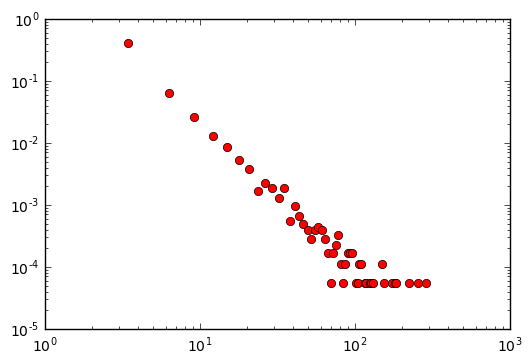
\includegraphics[height=0.4\textheight]{in-degree-distribution}
\end{figure}
\begin{figure}[!h]
\caption{توزیع تجمعی درجه ورودی}
\centering
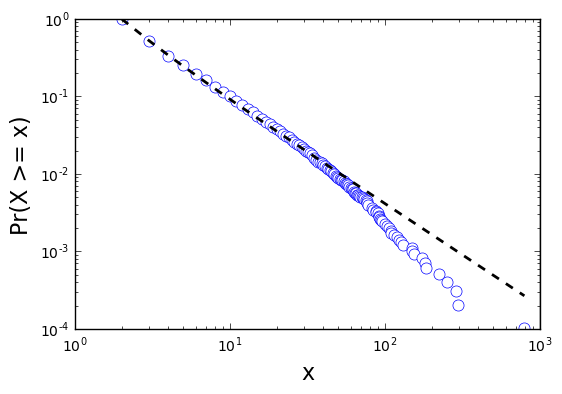
\includegraphics[height=0.4\textheight]{in-degree-distribution-exponent}
\end{figure}
\begin{figure}[!h]
\caption{رابطه ضریب خوشه‌بندی با درجه راس}
\centering
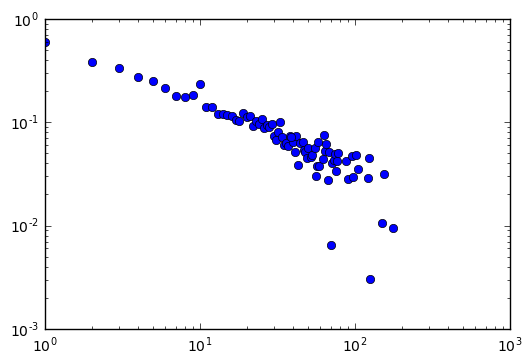
\includegraphics[height=0.4\textheight]{coeffition-degree}
\end{figure}
\begin{figure}[!h]
\caption{توزیع فاصله رئوس}
\centering
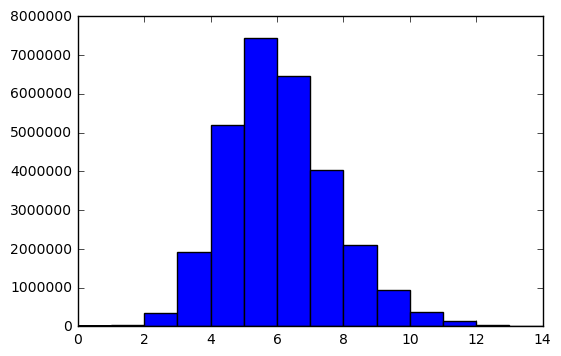
\includegraphics[height=0.4\textheight]{path-length}
\end{figure}
\begin{figure}[!h]
\caption{توزیع اندازه همه‌ی خوشه‌ها}
\centering
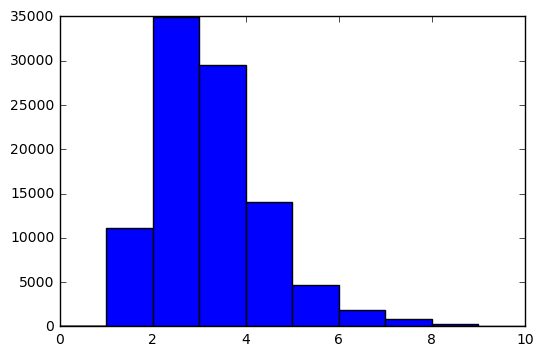
\includegraphics[height=0.4\textheight]{clique_count}
\end{figure}
\end{document}
